% !TEX TS-program = pdflatex
% !TEX encoding = UTF-8 Unicode

% This file is a template using the "beamer" package to create slides for a talk or presentation
% - Giving a talk on some subject.
% - The talk is between 15min and 45min long.
% - Style is ornate.

% MODIFIED by Jonathan Kew, 2008-07-06
% The header comments and encoding in this file were modified for inclusion with TeXworks.
% The content is otherwise unchanged from the original distributed with the beamer package.

\documentclass[handout]{beamer}


% Copyright 2004 by Till Tantau <tantau@users.sourceforge.net>.
%
% In principle, this file can be redistributed and/or modified under
% the terms of the GNU Public License, version 2.
%
% However, this file is supposed to be a template to be modified
% for your own needs. For this reason, if you use this file as a
% template and not specifically distribute it as part of a another
% package/program, I grant the extra permission to freely copy and
% modify this file as you see fit and even to delete this copyright
% notice. 


\mode<presentation>
{
  \usetheme{Warsaw}
  % or ...

  \setbeamercovered{transparent}
  % or whatever (possibly just delete it)
}


\usepackage[english]{babel}
% or whatever

\usepackage[utf8]{inputenc}
% or whatever

\usepackage{times}
\usepackage[T1]{fontenc}
% Or whatever. Note that the encoding and the font should match. If T1
% does not look nice, try deleting the line with the fontenc.

%%% MATH RELATED


%%% AMS math stuff
\usepackage{amsmath}
\usepackage{amssymb}
\usepackage{amsthm}
\usepackage{mathrsfs}
\usepackage{enumerate}

%%% Theorem environments
\newtheorem{thm}{Theorem}[subsection]
\newtheorem{prop}[thm]{Proposition}
\newtheorem{cor}{Corollary}[thm]
\newtheorem{por}[thm]{Porism}
\newtheorem{lem}[thm]{Lemma}
\theoremstyle{definition}
\newtheorem{prob}[thm]{Problem}
\newtheorem{soln}{Solution}
\newtheorem{defn}[thm]{Definition}
\newtheorem{ex}[thm]{Example}
\newtheorem{quest}[thm]{Question}
\newtheorem{remk}[thm]{Remark}

%%% Typesetting shortcuts
\newcommand{\tn}[1]{\textnormal{#1}}
\newcommand{\ol}[1]{\overline{#1}}
\newcommand{\wt}[1]{\widetilde{#1}}
\newcommand{\wh}[1]{\widehat{#1}}
\newcommand{\vocab}[1]{\textbf{#1}\index{#1}}

%%% Math shortcuts
\newcommand{\bbr}{\mathbb R}
\newcommand{\bbz}{\mathbb Z}
\newcommand{\bbq}{\mathbb Q}
\newcommand{\bbn}{\mathbb N}
\newcommand{\bbf}{\mathbb F}
\newcommand{\bbc}{\mathbb C}
\newcommand{\bbd}{\mathbb D}
\newcommand{\bba}{\mathbb A}
\newcommand{\bbp}{\mathbb P}
\newcommand{\bbg}{\mathbb G}
\newcommand{\bbv}{\mathbb V}
\newcommand{\dih}[1]{\mathcal D_{#1}}
\newcommand{\sym}[1]{\mathcal S_{#1}}
\newcommand{\vspan}{\tn{span}}
\newcommand{\trace}{\tn{trace}}
\newcommand{\diff}{\backslash}
\newcommand{\stab}{\tn{stab}}
\newcommand{\conv}{\tn{conv}}
\newcommand{\img}{\tn{img}}
\newcommand{\coker}{\tn{coker}}
\newcommand{\id}{\tn{id}}
\newcommand{\Hom}{\tn{Hom}}
\newcommand{\End}{\tn{End}}
\newcommand{\Aut}{\tn{Aut}}
\newcommand{\aut}{\tn{Aut}}
\newcommand{\ann}{\tn{Ann}}
\newcommand{\GL}{\tn{GL}}
\newcommand{\Gr}{\tn{Gr}}
\newcommand{\lord}{\preccurlyeq}
\newcommand{\rord}{\succcurlyeq}
\newcommand{\tr}{\textnormal{Tr}}
\newcommand{\Tr}{\textnormal{Tr}}
\newcommand{\bbl}{\mathbb{L}}
\newcommand{\C}{\mathscr{C}}
\newcommand{\X}{\mathscr{X}}
\renewcommand{\S}{\mathscr{S}}
\newcommand{\M}{\mathscr{M}}
\renewcommand{\L}{\mathcal{L}}


%%% Algebraic Geometry
\newcommand{\height}{\textnormal{ht}}
\newcommand{\A}{\mathbb{A}}
\newcommand{\p}{\mathfrak{p}}
\newcommand{\sheaf}[1]{\mathcal{#1}}
\newcommand{\spec}{\textnormal{Spec}}
\newcommand{\proj}{\textnormal{Proj}}
\newcommand{\Aff}{\textnormal{Aff}}
\newcommand{\skel}{\textnormal{skel}}
\newcommand{\supp}{\textnormal{supp}}
\newcommand{\orb}{\textnormal{orb}}
\newcommand{\Proj}{\textnormal{Proj}}
\newcommand{\Pic}{\textnormal{Pic}}
\newcommand{\Rees}{\textnormal{Rees}}
\newcommand{\shom}{\mathcal{H}om}

\renewcommand*\arraystretch{1.3}

%%% paper specific definitions
\newcommand{\weyl}{\Omega}
\newcommand{\weyll}{{\widehat{\Omega}}}
\newcommand{\weylll}{{\widetilde{\Omega}}}
\newcommand{\mweyl}{{M_N(\Omega)}}
\newcommand{\mweyll}{{M_N(\widehat{\Omega})}}
\newcommand{\mweylll}{{M_N(\widetilde{\Omega})}}
\newcommand{\seq}{\text{Seq}}
\newcommand{\tail}{\text{Tail}}
\newcommand{\Ad}{\textnormal{Ad}}
\newcommand{\sech}{\textnormal{sech}}
\newcommand{\colim}{\varinjlim}
\newcommand{\limit}{\varprojlim}
\newcommand{\Bis}{\textnormal{Bis}}
\newcommand{\m}{\mathfrak{m}}
\newcommand{\mxx}[4]{\left(\begin{array}{cc} #1 & #2\\ #3 & #4 \end{array}\right)}
\newcommand{\diag}{\text{diag}}
\newcommand{\qdet}{\textnormal{qdet}}
\newcommand{\mdet}{\textnormal{mdet}}
\newcommand{\mtau}{\mathcal{T}}
\newcommand{\cof}{\textnormal{cof}}
\newcommand{\minor}{\textnormal{minor}}
\newcommand{\holo}{Holo}
\newcommand{\ord}{\textnormal{order}}
\newcommand{\mult}{\mathfrak M}






\title{Computational Linear Algebra HYPE!!} 
\subtitle
{} % (optional)

\author[W.R. Casper] % (optional, use only with lots of authors)
{W.R. Casper}
% - Use the \inst{?} command only if the authors have different
%   affiliation.

\institute[California State University Fullerton] % (optional, but mostly needed)
{
  Department of Mathematics\\
  California State University Fullerton}
% - Use the \inst command only if there are several affiliations.
% - Keep it simple, no one is interested in your street address.

\subject{Talks}
% This is only inserted into the PDF information catalog. Can be left
% out. 



% If you have a file called "university-logo-filename.xxx", where xxx
% is a graphic format that can be processed by latex or pdflatex,
% resp., then you can add a logo as follows:

% \pgfdeclareimage[height=0.5cm]{university-logo}{university-logo-filename}
% \logo{\pgfuseimage{university-logo}}



% Delete this, if you do not want the table of contents to pop up at
% the beginning of each subsection:
%\AtBeginSubsection[]
%{
%  \begin{frame}<beamer>{Outline}
%    \tableofcontents[currentsection,currentsubsection]
%  \end{frame}
%}


% If you wish to uncover everything in a step-wise fashion, uncomment
% the following command: 

%\beamerdefaultoverlayspecification{<+->}


\begin{document}

\begin{frame}
  \titlepage
\end{frame}

%\begin{frame}{Outline}
%  \tableofcontents
%  % You might wish to add the option [pausesections]
%\end{frame}

% Since this a solution template for a generic talk, very little can
% be said about how it should be structured. However, the talk length
% of between 15min and 45min and the theme suggest that you stick to
% the following rules:  

% - Exactly two or three sections (other than the summary).
% - At *most* three subsections per section.
% - Talk about 30s to 2min per frame. So there should be between about
%   15 and 30 frames, all told.

\section{Applications of Computational Linear Algebra}
\subsection{Let's get hyped!!}
\begin{frame}{}
 \begin{columns}
  \column{0.38\linewidth}
    \centering
             
\includegraphics[width=\linewidth]{img/hype.jpg}
  \column{0.62\linewidth}
    \begin{itemize}
      \item linear algebra is used in almost any other math!
      \item tons of real-world applications
      \item most important math classes of your undergraduate career -- and you get to start your \textbf{first year}!!
      \item computer programming is incredibly powerful
      \item can store and process huge amounts of data, perform computations quickly, automate, ...
      \item put together you can solve many real world problems
    \end{itemize}
 \end{columns} 
\end{frame}

\begin{frame}{}
 \begin{columns}
  \column{0.38\linewidth}
    \centering
             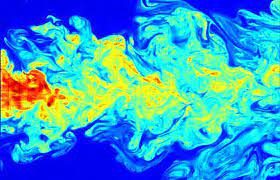
\includegraphics[width=1.5\linewidth,angle=90]{img/cfd.jpg}
  \column{0.62\linewidth}
    \begin{itemize}
      \item think about a fast, hot stream of water in the ocean
      \item fluid dynamics are beautiful and complicated
      \item fluid flows are determined by differential equations
      \item can be modelled on a computer with linear algebra!
    \end{itemize}
 \end{columns} 
\end{frame}

\begin{frame}{}
 \begin{columns}
  \column{0.38\linewidth}
    \centering
             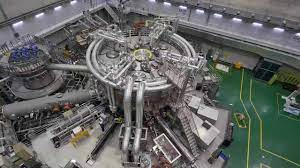
\includegraphics[width=\linewidth]{img/fusion1.jpg}
	     \\\vspace{.3in}
             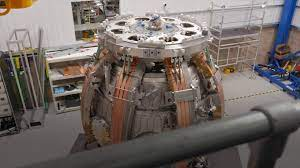
\includegraphics[width=\linewidth]{img/fusion2.jpg}
  \column{0.62\linewidth}
    \begin{itemize}
      \item think about designing a fission reactor
      \item a somewhat important question is will it explode?
      \item depends on absorbtion/emission of neutrons in reactor
      \item governed by neutron transport equations
      \item we can use computational linear algebra to find out if it's safe before building it
    \end{itemize}
 \end{columns} 
\end{frame}

\begin{frame}{}
 \begin{columns}
  \column{0.38\linewidth}
    \centering
             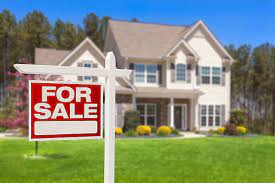
\includegraphics[width=\linewidth]{img/forsale.jpg}
  \column{0.62\linewidth}
    \begin{itemize}
      \item you are selling your home
      \item how much is reasonable to ask for?
      \item can look at prices of many other homes sold in neighborhood
      \item compare bedrooms, bathrooms, square footage, amenities, etc
      \item use linear regression on a computer to predict price
    \end{itemize}
 \end{columns} 
\end{frame}

\begin{frame}{}
 \begin{columns}
  \column{0.38\linewidth}
    \centering
             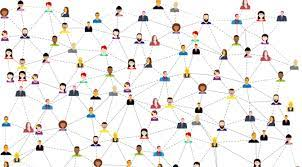
\includegraphics[width=\linewidth]{img/social-network.jpg}
	     \\\vspace{.3in}
             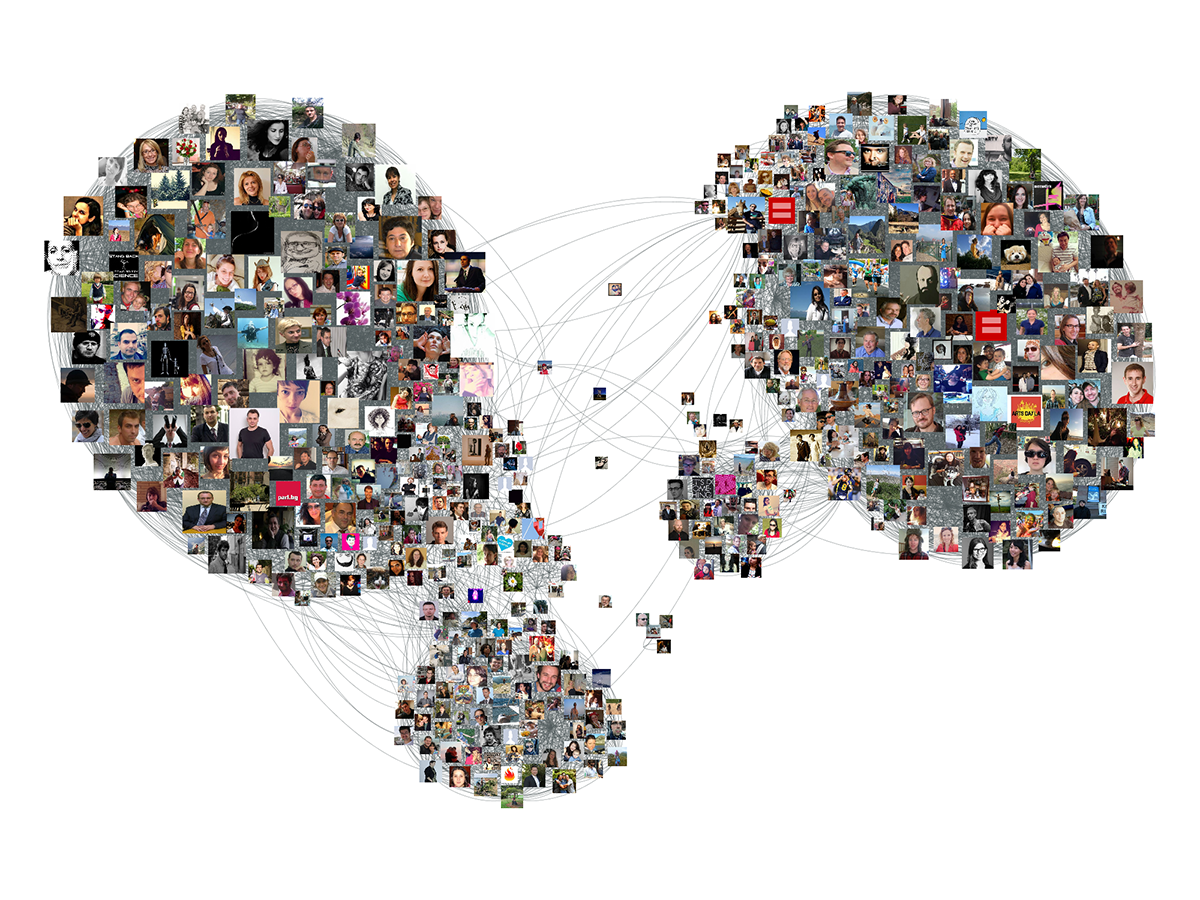
\includegraphics[width=\linewidth]{img/facebook.png}
  \column{0.62\linewidth}
    \begin{itemize}
      \item imagine a social network (Facebook, Reddit, etc.)
      \item connect people if they are ``friends''
      \item can we predict who may actually hang out in real life?
      \item can we find common properties which accurately predict friendships?
      \item can use computational linear algebra to do this!
    \end{itemize}
 \end{columns} 
\end{frame}

\begin{frame}{}
 \begin{columns}
  \column{0.38\linewidth}
    \centering
             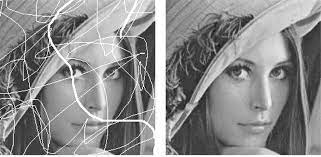
\includegraphics[width=\linewidth]{img/image-processing.jpg}
	     \\\vspace{.3in}
             
\includegraphics[width=\linewidth]{img/filters.jpg}
  \column{0.62\linewidth}
    \begin{itemize}
      \item you can use computational linear algebra to touch up a damaged photo
      \item computational linear algebra is also behind popular image filters on Snapchat and Instagram
    \end{itemize}
 \end{columns} 
\end{frame}

\begin{frame}{}
 \begin{columns}
  \column{0.38\linewidth}
    \centering
             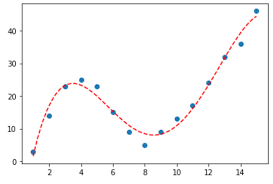
\includegraphics[width=\linewidth]{img/curve-fitting.png}
	     \\\vspace{.3in}
             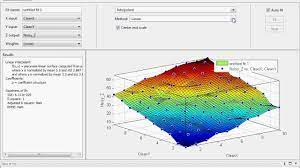
\includegraphics[width=\linewidth]{img/curve-fitting-2d.jpg}
  \column{0.62\linewidth}
    \begin{itemize}
      \item suppose you experimentally measure a bunch of data
      \item you know your data should fit a particular pattern (like a polynomial)
      \item your actual measurements won't be exactly because of measurement errors
      \item you can use computational linear algebra to find the curve which most closely fits the data
    \end{itemize}
 \end{columns} 
\end{frame}



\end{document}


